\documentclass{article}
% Language setting
% Replace `english' with e.g. `spanish' to change the document language
\usepackage{biblatex} %Imports biblatex package
\addbibresource{sample.bib}
\usepackage{changepage}
\usepackage[english]{babel}
\usepackage{tikz}
\usepackage{array}
\usepackage{amsmath}
\usepackage{accents}
\usepackage{empheq}
\usepackage{pythonhighlight}
\newcolumntype{P}[1]{>{\centering\arraybackslash}p{#1}}
\newcolumntype{M}[1]{>{\centering\arraybackslash}m{#1}}

% Set page size and margins
% Replace `letterpaper' with `a4paper' for UK/EU standard size
\usepackage[letterpaper,top=2cm,bottom=2cm,left=3cm,right=3cm,marginparwidth=1.75cm]{geometry}

\usepackage{graphicx}
\usepackage[colorlinks=true, allcolors=blue]{hyperref}
\usepackage{setspace}
\usepackage{booktabs}
\usepackage[T1]{fontenc}
\usepackage{longtable}
\doublespacing

\begin{document}
\newcommand{\circled}[1]{\tikz[baseline=(char.base)]{
            \node[shape=circle,draw,inner sep=2pt] (char) {#1};}}
\begin{titlepage}

\centering
\scshape
\vspace{\baselineskip}

%
\rule{\textwidth}{1.6pt}\vspace*{-\baselineskip}\vspace*{2pt}
\rule{\textwidth}{0.4pt}

{\Huge \textbf{\textsc{NPRE 449: Homework 3 \\
\vspace{15pt}}}}

\rule{\textwidth}{0.4pt}\vspace*{-\baselineskip}\vspace{3.2pt}
\rule{\textwidth}{1.6pt}\vspace{6pt}
%%\centerline{\textit{University of Illinois at Urbana-Champaign}} 
\vspace{1.5\baselineskip}


\large \centerline{\textbf{Author:} Nathan Glaser}
\large \centerline{\textbf{Net-ID:} nglaser3}
\quad

\vfill
\large \centerline{September 18, 2024}
%
\pagenumbering{gobble}
\end{titlepage}

\tableofcontents
\newpage
\pagenumbering{arabic}

\newcommand{\leftrightharpoonup}{\mathrel{\mathpalette\lrhup\relax}}
\newcommand{\lrhup}[2]{\ooalign{$#1\leftharpoonup$\cr$#1\rightharpoonup$\cr}}
\newcommand{\pd}[3]{\frac{\partial^{#3}#1}{\partial#2^{#3}}}
\newcommand{\phase}{\left(\Vec{r},t\right)}
\newcommand*\vect[1]{\mkern2mu\accentset{\rightharpoonup}{#1}\mkern2mu}
\newcommand*\tensor[1]{\mkern2mu\accentset{\leftrightharpoonup}{#1}\mkern2mu}
\renewcommand{\Vec}[1]{\vect{#1}}
\newcommand{\stress}{\tensor{\mathbf{\tau}}}

\newcommand{\mass}{\pd{\rho}{t}{} + \nabla\cdot\rho\Vec{v} = 0}
\newcommand{\momentum}{\pd{\rho\Vec{v}}{t}{} + \nabla \cdot \rho\Vec{v}\Vec{v}=-\nabla P + \nabla \cdot \stress+\rho \Vec{g}}
\newcommand{\energy}{\pd{\rho u}{t}{} + \nabla\cdot\rho\Vec{v}u 
        =
        -\nabla\cdot q'' - P\nabla\cdot\Vec{v} + \stress\mathbf{:}\nabla\Vec{v}+q'''}
        
\section*{Question 1}
\addcontentsline{toc}{section}{\protect\numberline{}Question 1}
To begin, the Navier-Stokes equations are:

\begin{subequations}
    \begin{equation}
        \mass
        \label{mass}
    \end{equation}
    \begin{equation}
        \momentum
        \label{momentum}
    \end{equation}
    \begin{equation}
        \energy
        \label{energy}
    \end{equation}
\end{subequations}


First, we expand the mass equation into Cartesian coordinates. This is rather rudimentary as the mass equation is a scalar equation, and there is only the divergence of a vector to be done:
\begin{equation}
    \begin{gathered}
        \mass \\
        \pd{\rho}{t}{} + \left[\pd{\rho v_x}{x}{} + \pd{\rho v_y}{y}{} + \pd{\rho v_z}{z}{}\right] = 0\\
    \end{gathered}
\end{equation}

And so, for the mass equation:
\begin{equation}
    \boxed{\pd{\rho}{t}{} + \left[\pd{\rho v_x}{x}{} + \pd{\rho v_y}{y}{} + \pd{\rho v_z}{z}{}\right] = 0}
    \label{cartmass}
\end{equation}

Next, the momentum equation. To do this we will break into x, y, and z equations, as the momentum equation is a vector equation. The equations x, y, and z will all have the same form just with different subscripts. The expansion will be done with x. So as to not have a multi-line equation, each term will be defined for specifically x. To do this various steps are undertaken. Firstly, the divergence of $\Vec{v}\Vec{v}$ can be seen as, in the x direction, $\nabla (v_x\Vec{v})$. Next, the pressure is simply just the derivative of pressure in the x direction. Then, the divergence of the stress tensor is functionally similair to the divergence of the vector-vector multiplication, $\nabla \stress_x$. Finally, the gravity form is simply the x-component of g.

\newcommand{\mompvv}[1]{\pd{\rho v_{#1}v_x}{x}{} + \pd{\rho v_{#1} v_y}{y}{} + \pd{\rho v_{#1} v_z}{z}{}}
\newcommand{\momP}[1]{\pd{P_{#1}}{#1}{}}
\newcommand{\momds}[1]{\pd{\stress_{#1 x}}{x}{} + \pd{\stress_{#1 y}}{y}{} + \pd{\stress_{#1 z}}{z}{}}
\newcommand{\momg}[1]{\rho g_{#1}}
\newcommand{\mom}[1]{
\pd{\rho v_{#1}}{t}{} + \left[\mompvv{#1}\right] = -\momP{#1} + \left[\momds{#1}\right] +\momg{#1}
}
\begin{equation}
\begin{gathered}
    \nabla \cdot \rho\Vec{v}\Vec{v} = \mompvv{x} \\ 
    \nabla P = \momP{x}\\
    \nabla \cdot \stress = \momds{x}\\
    \rho \Vec{g} = \momg{x}
\end{gathered}
\end{equation}

\newpage
Substituting these into our seperated momentum equations, we get the momentum equation expanded into x, y, and z:
\begin{subequations}
    \begin{equation}
        \boxed{\mom{x}}
    \end{equation}
    \begin{equation}
        \boxed{\mom{y}}
    \end{equation}
    \begin{equation}
        \boxed{\mom{z}}
    \end{equation}
\end{subequations}

Finally, for the energy equation. This is fortunately a scalar equation, and is thus not needed to be separated into different equations. First, $\nabla\cdot \rho\Vec{v}u$ is simply the divergence of a vector, in which each component is multiplied by $\rho$ and $u$. Next, $\nabla \cdot q''$ is again just the divergence of the $q''$ vector. Further, $P\nabla\cdot\Vec{v}$ is again just the divergence of a vector multiplied by the pressure.

\newcommand{\enpvu}{\pd{\rho v_x u}{x}{} + \pd{\rho v_y u}{y}{} + \pd{\rho v_z u}{z}{}}
\newcommand{\enqpp}{\pd{q_{x}''}{x}{} + \pd{q_y''}{y}{} + \pd{q_z''}{z}{}}
\newcommand{\enpdv}{P\left[\pd{v_x}{x}{} + \pd{v_y}{y}{} + \pd{v_z}{z}{}\right]}

\begin{equation}
    \begin{gathered}
        \nabla\cdot \rho\Vec{v}u = \enpvu\\
        \nabla \cdot q'' = \enqpp\\
        P\nabla\cdot\Vec{v} = \enpdv
    \end{gathered}
\end{equation}

Then to explain the $\stress:\nabla\Vec{v}$. First, the $\nabla\Vec{v}$. This is actually written as $\nabla^T\Vec{v}$:

\begin{equation}
    \nabla^T\Vec{v} = 
    \begin{bmatrix}
        \pd{}{x}{}\\
        \pd{}{y}{}\\
        \pd{}{z}{}
    \end{bmatrix}
    \left[v_x \:\: v_y \:\: v_z \right] = 
    \begin{bmatrix}
        \pd{v_x}{x}{} \:\:\pd{v_x}{y}{} \:\:\pd{v_x}{z}{} \\
        \pd{v_y}{x}{} \:\:\pd{v_y}{y}{} \:\:\pd{v_y}{z}{} \\
        \pd{v_z}{x}{} \:\:\pd{v_z}{y}{} \:\:\pd{v_z}{z}{}
    \end{bmatrix}
\end{equation}

Thus the double dot product has the true form of:

\begin{equation}
    \stress:\nabla\Vec{v}=
    \begin{bmatrix}
        \tau_{ii} \:\: \tau_{ij} \:\: \tau_{ik} \\
        \tau_{ji} \:\: \tau_{jj} \:\: \tau_{kk} \\
        \tau_{ki} \:\: \tau_{kj} \:\: \tau_{kk}
    \end{bmatrix}
    :
    \begin{bmatrix}
        \pd{v_x}{x}{} \:\:\pd{v_x}{y}{} \:\:\pd{v_x}{z}{} \\
        \pd{v_y}{x}{} \:\:\pd{v_y}{y}{} \:\:\pd{v_y}{z}{} \\
        \pd{v_z}{x}{} \:\:\pd{v_z}{y}{} \:\:\pd{v_z}{z}{}
    \end{bmatrix}
\end{equation}

Next, the double dot product of two tensors is very similair to a vector dot product. Each component in the tensor will be multiplied by its corresponding component in the other tensor, then all of the products will be summed.
\begin{multline}
    \stress:\nabla\Vec{v}= 
    \tau_{ii}\pd{v_x}{x}{} + \tau_{ij}\pd{v_x}{y}{} + \tau_{ik}\pd{v_x}{z}{} + 
    \tau_{ji}\pd{v_y}{x}{} + \tau_{jj}\pd{v_y}{y}{} + \tau_{jk}\pd{v_y}{z}{} +
    \tau_{ki}\pd{v_z}{x}{} + \tau_{kj}\pd{v_z}{y}{} + \tau_{kk}\pd{v_z}{z}{}
\end{multline}

Or, in shorter notation (where i, j, k are x, y, z):

\newcommand{\energydoubledot}{\sum_{n}^{i,j,k}\:\sum_{m}^{i,j,k} \tau_{nm}\pd{v_n}{m}{}}
\begin{equation}
    \stress:\nabla\Vec{v} = \sum_{n}^{i,j,k}\:\sum_{m}^{i,j,k} \tau_{nm}\pd{v_n}{m}{}
\end{equation}

Finally, we can plug these all back into our energy equation, yielding the energy equation expanded into Cartesian. Both the short-hand and long form are presented. Short form:
\begin{multline}
    \pd{\rho u}{t}{} + \left[\enpvu\right] = -\left[\enqpp\right]\\ -\enpdv + \energydoubledot + q'''
\end{multline}

Long form:
\begin{empheq}[box=\fbox]{multline}
    \pd{\rho u}{t}{} + \left[\enpvu\right] = -\left[\enqpp\right]\\
    -\enpdv + q''' + 
    \biggl[\tau_{ii}\pd{v_x}{x}{} + \tau_{ij}\pd{v_x}{y}{} + \tau_{ik}\pd{v_x}{z}{}  \\ 
    +\tau_{ji}\pd{v_y}{x}{} + \tau_{jj}\pd{v_y}{y}{} + \tau_{jk}\pd{v_y}{z}{} +
    \tau_{ki}\pd{v_z}{x}{} + \tau_{kj}\pd{v_z}{y}{} + \tau_{kk}\pd{v_z}{z}{}\biggr]
\end{empheq}


\newpage
\section*{Question 2}
\addcontentsline{toc}{section}{\protect\numberline{}Question 2}

From our assumptions, the mass and momentum equations simplify, in cylindrical coordinates, to:

\begin{subequations}
    \begin{equation}
        \nabla\cdot\Vec{v} = 0
    \end{equation}
    \begin{equation}
        0 = -\pd{P}{r}{} + \rho g_r
    \end{equation}
    \begin{equation}
        0 = -\frac{1}{r}\pd{P}{\theta}{} + \rho g_{\theta}
    \end{equation}
    \begin{equation}
        0 = -\pd{P}{z}{} + \mu \left[ \frac{1}{r}\pd{}{r}{}r\pd{v_z}{r}{} \right]
    \end{equation}
\end{subequations}

Finally the energy equation simplifies as follows, because specific internal energy $u$ is simply $c_pT$:
\begin{subequations}
    \begin{equation}
        \nabla\cdot\rho\Vec{v}u = -\nabla\cdot\Vec{q}''
    \end{equation}    
    \begin{equation}
        \rho c_p\left[ \frac{1}{r}\pd{}{r}{}(rv_rT) + \frac{1}{r}\pd{v_{\theta}T}{\theta}{} + \pd{v_zT}{z}{}\right] = k\left[\frac{1}{r}\pd{}{r}{}r\pd{T}{r}{} +\frac{1}{r^2}\pd{T}{\theta}{2} + \pd{T}{z}{2}\right]
    \end{equation}
    \begin{equation}
        v_z\pd{T}{z}{} = \frac{k}{\rho c_p} \frac{1}{r}\pd{}{r}{}r\pd{T}{r}{}
    \end{equation}
\end{subequations}

Finally we can solve these equations for axial velocity and temperature. 

First, we will solve for the pressure profile. We know that $\Vec{g}$ is equal to $\langle -g\sin(\theta), \: -g\cos(\theta), \: 0\rangle$. Thus:

\begin{subequations}
    \begin{equation}
        P = -\rho g r \sin{\theta} + C(\theta, z)
    \end{equation}
    \begin{equation}
        P = -\rho g r \sin\theta + C(r, z)
    \end{equation}
\end{subequations}

And because the result from both radial and azimuthal solving yields the same functional form, we know that $C$ must only be a function of z. Further, we know that pressure must be a linear function of z, as its derivative with respect to z must not be a function of z. Thus, we can solve for the velocity profile. 

\begin{subequations}
    \begin{equation}
        \frac{P_0r}{\mu} = \pd{}{r}{}r\pd{v_z}{r}{}
    \end{equation}
    \begin{equation}
        \frac{P_0r}{2\mu} +\frac{C_1}{r}= \pd{v_z}{r}{}
    \end{equation}
    \begin{equation}
        v_z(r) = \frac{P_0r^2}{4\mu} + C_1\ln r + C_2
    \end{equation}
\end{subequations}

\newpage
Next for our boundary conditions:
\begin{itemize}
    \item[\circled{1}] No-Slip Condition: $v_z(R_o) = 0$
    \item[\circled{2}] Symmetry: $\pd{v_z(0)}{r}{}=0$, or Finiteness at the centerline
\end{itemize}
Thus, $C_1$ must be 0 by \circled{2}, and then investigating \circled{1}, $C_2$ must be:
\begin{subequations}
    \begin{equation}
        v_z(R_0) = \frac{P_0R_0^2}{4\mu} + C = 0
    \end{equation}
    \begin{equation}
        C = -\frac{P_0R_0^2}{4\mu}
    \end{equation}
\end{subequations}

Thus our axial velocity, recognizing that $P_0 = \frac{-\Delta P}{l}$, is:
\begin{equation}
    v_z(r) = \frac{\Delta PR^2}{4\mu l} -\frac{\Delta P r^2}{4\mu l} = \frac{\Delta P}{4\mu l}(R^2-r^2) = \langle v_z\rangle (1-\frac{r^2}{R^2})
\end{equation}
Such that $\langle v_z \rangle = \frac{\Delta PR^2}{4\mu l}$. 

Now, for the temperature. Importantly, $\pd{T}{z}{}$ is a constant because of the definition of fully developed temperature flow. .
\newcommand{\vz}{\langle v_z \rangle}
\newcommand{\lhcrud}{\frac{\vz\ \rho\ c_p}{k}\pd{T}{z}{}}
\begin{subequations}
    \begin{equation}
        v_z(r)\pd{T}{z}{} = \frac{k}{\rho c_pr}\pd{}{r}{}r\pd{T}{r}{}
    \end{equation}
    \begin{equation}
         \lhcrud (r-\frac{r^3}{R^2}) = \pd{}{r}{}r\pd{T}{r}{}
    \end{equation}
    \begin{equation}
        \lhcrud (\frac{r}{2}-\frac{r^3}{4R^2}) +\frac{C_1}{r}= \pd{T}{r}{}
    \end{equation}
    \begin{equation}
        T(r,z) = \lhcrud \left[\frac{r^2}{4}-\frac{r^4}{16R^2}\right] + C_1 \ln(r) + C_2
    \end{equation}
\end{subequations}

And then again for simplicity, I define $\lhcrud$ as equal to $\xi$:
\begin{equation}
    T(r,z) = \xi \left[\frac{r^2}{4}-\frac{r^4}{16R^2}\right] + C_1 \ln(r) + C_2
\end{equation}

\newpage
Now for our boundary conditions:

\begin{itemize}
    \item[\circled{1}] Symmetry: $\pd{T(0)}{r}{}$, or Finiteness at the center line
    \item[\circled{2}]  $T(R,z) = T_s(z)$
\end{itemize}

Investigating \circled{1}, $C_1$ must be 0. Then from \circled{2}:
\begin{subequations}
    \begin{equation}
        T(R,z) = \xi \left[\frac{R^2}{4}-\frac{R^2}{16}\right] + C_2
    \end{equation}
    \begin{equation}
        T_s(z) - \xi \left[\frac{3R^2}{16}\right] = C_2
    \end{equation}
\end{subequations}

Thus, our temperature distribution is:
\begin{equation}
    T(r,z) = \xi \left[\frac{r^2}{4}-\frac{r^4}{16R^2}\right] + T_s(z) - \xi\frac{3R^2}{16}
\end{equation}

Then to find the normalized temperature, $\frac{T_s(z) - T(r,z)}{T_s(z) - T_{cl}(z)}$:
\begin{subequations}
    \begin{equation}
        T_s(z) - T(r,z) = \xi\left[ \frac{r^4}{16R^2} - \frac{r^2}{4} + \frac{3R^2}{16} \right]
    \end{equation}
    \begin{equation}
        T_s(z) - T_{cl}(z) = \xi [\frac{3R^2}{16}]
    \end{equation}
\end{subequations}

Thus:
\begin{subequations}

    \begin{equation}
        \frac{T_s(z) - T(r,z)}{T_s(z) - T_{cl}(z)} = \frac{\frac{r^4}{16R^2} - \frac{r^2}{4} + \frac{3R^2}{16}}{\frac{3R^2}{16}}
    \end{equation}
    \begin{equation}
        \frac{T_s(z) - T(r,z)}{T_s(z) - T_{cl}(z)} = \frac{r^4}{3R^4} - \frac{4r^2}{3R^2} + 1 
    \end{equation}
\end{subequations}

Finally, the normalized temperature and velocity distributions are:
\begin{figure}[!h!]
    \centering
    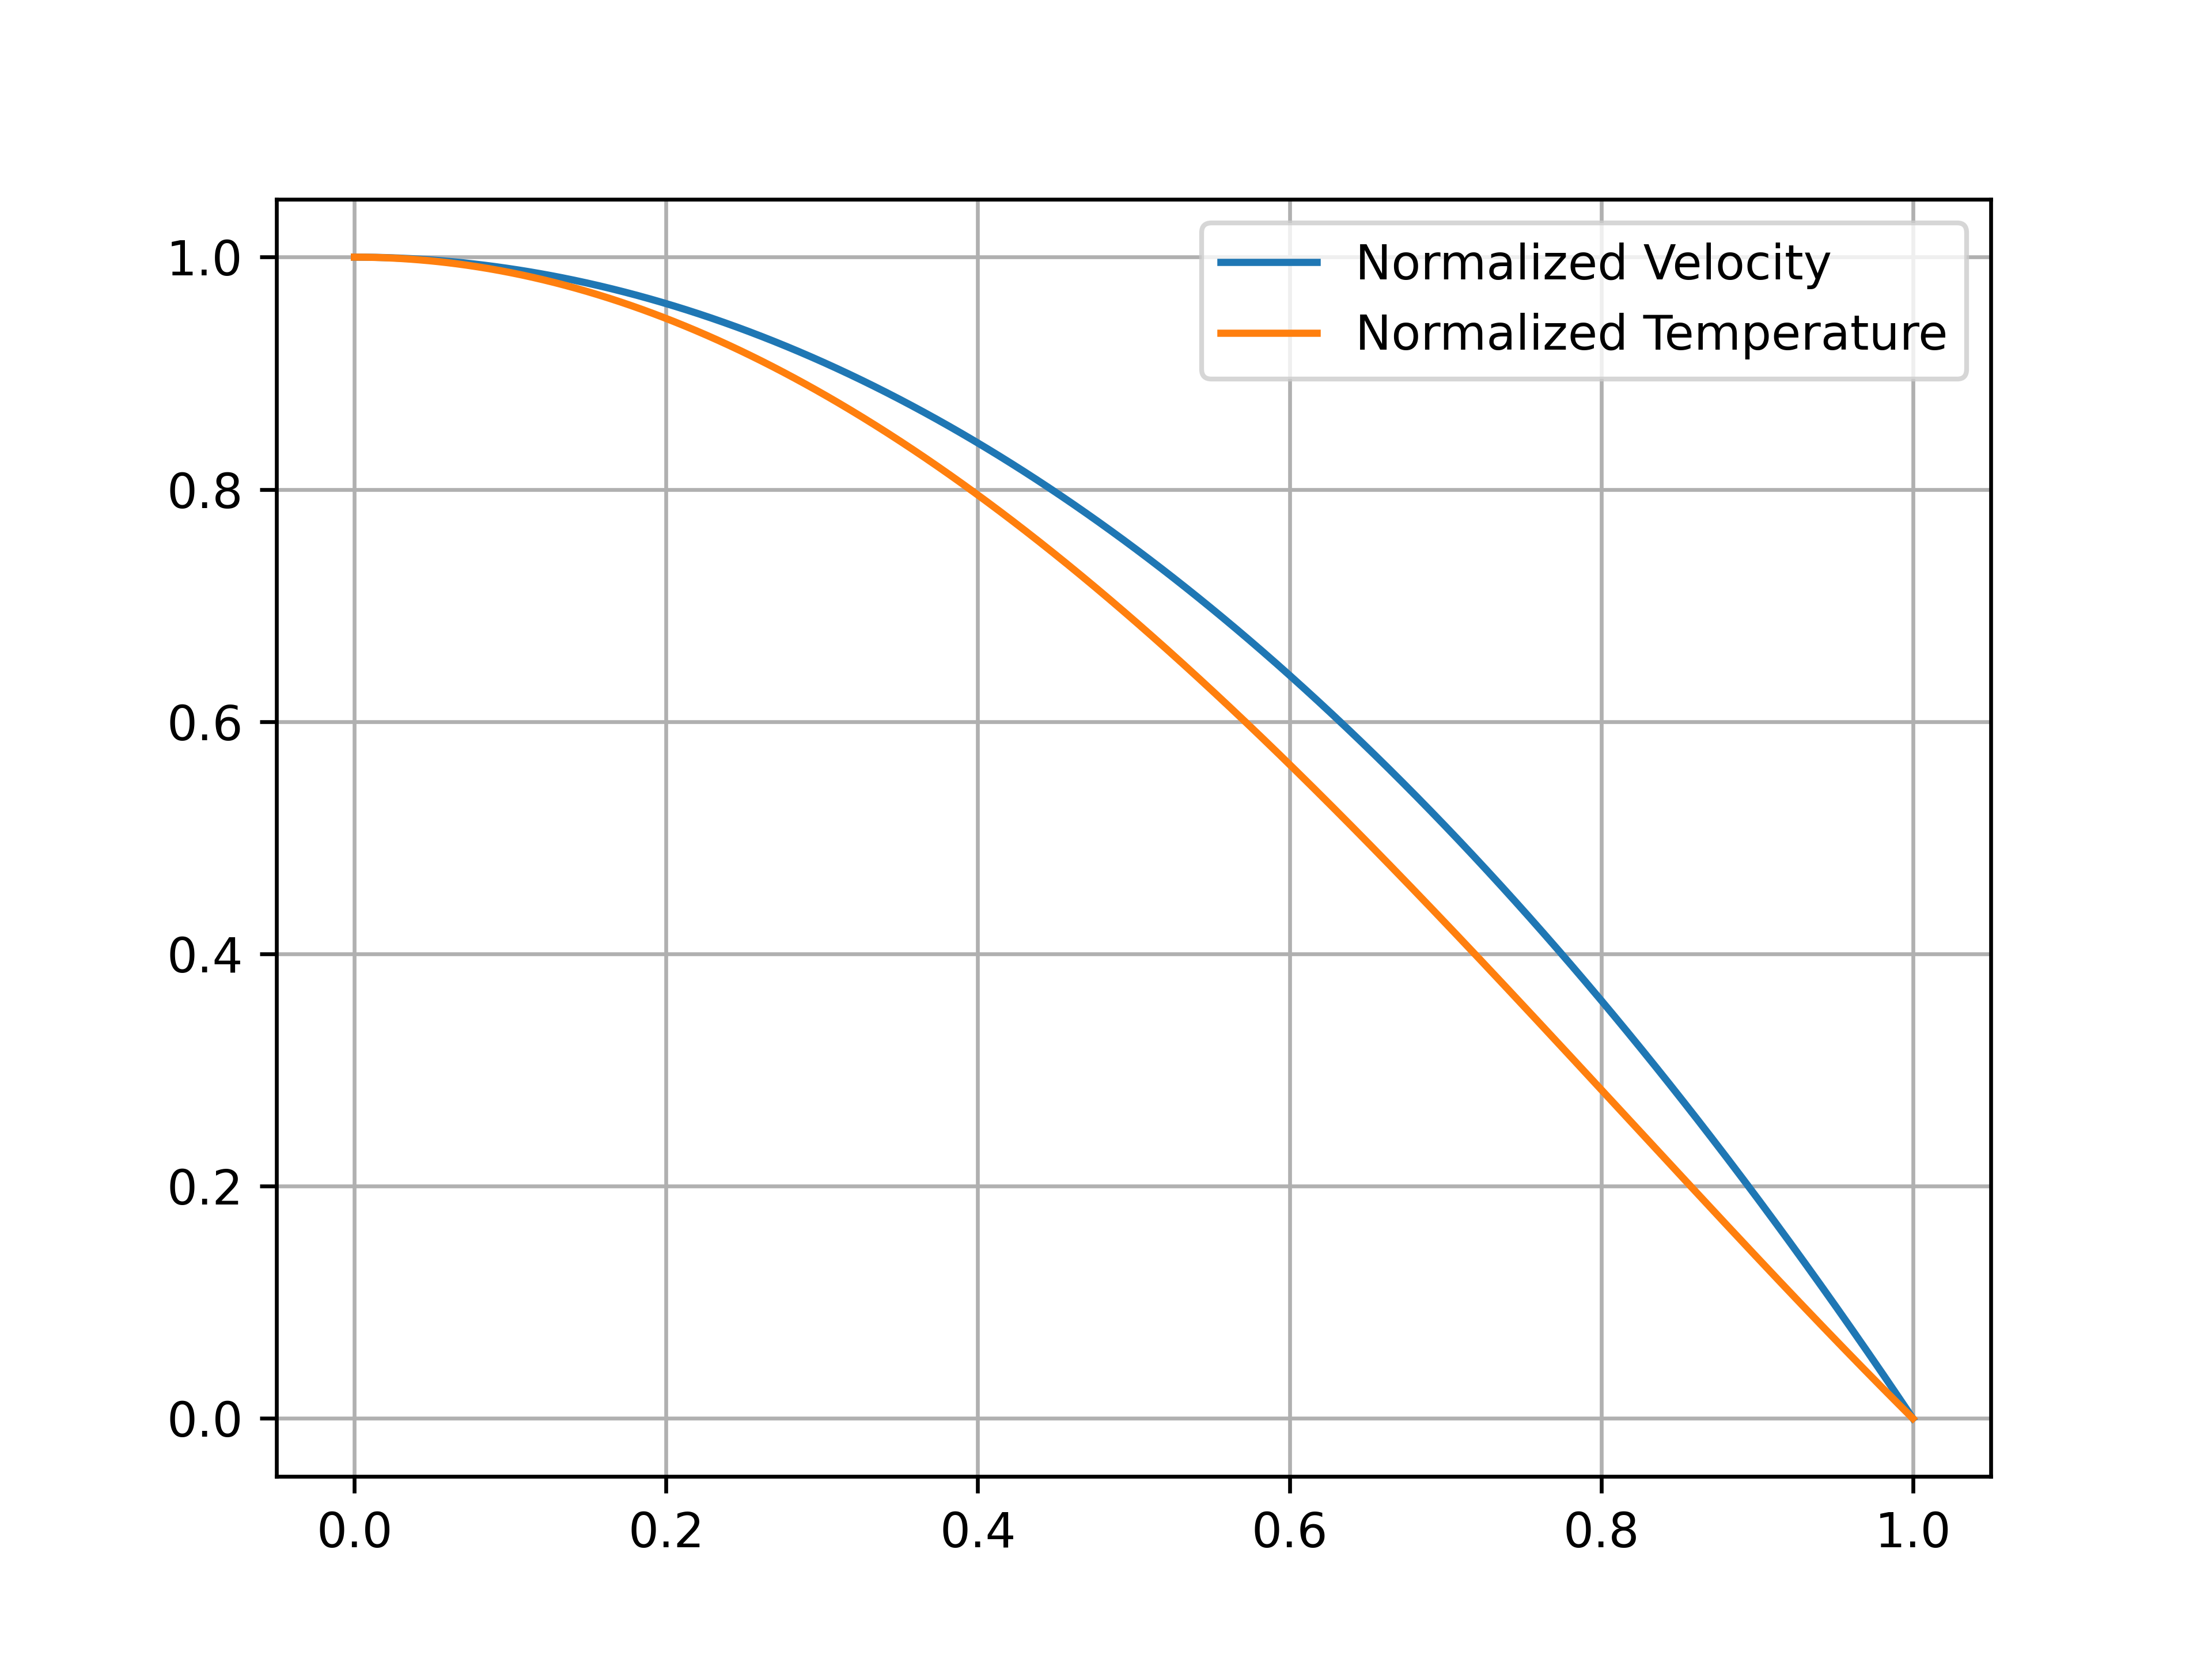
\includegraphics[width=0.5\linewidth]{plots/q2.png}
    \label{fig:q2}
\end{figure}

\newpage
\section*{Question 3}
\addcontentsline{toc}{section}{\protect\numberline{}Question 2}
To begin, we can skip all of the beginning cruft. We already know our velocity profile:

\begin{equation}
    v_z(r) = \frac{\Delta P}{4\mu\ l} (r^2 - R^2)
\end{equation}
And taking the area average of this:
\begin{subequations}
    \begin{equation}
        \vz = \frac{1}{\pi R^2}\int^{2\pi}_0\int_0^R r v_z(r) dr d\theta
    \end{equation}
    \begin{equation}
        \vz = \frac{1}{\pi R^2}\frac{\pi\Delta P}{2\mu l}(\frac{r^4}{4}-\frac{R^2r^2}{2})\biggr|^R_0
    \end{equation}
    \begin{equation}
        \vz = \frac{-R^2\Delta P}{8\mu l}
    \end{equation}
\end{subequations}

Thus, the velocity profile is equal to $2\vz (1-\frac{r^2}{R^2})$.

Next, our energy equation is: 
\begin{subequations}
    \begin{equation}
        \rho c_p v_z(r) \pd{T}{z}{} = \frac{k}{r}\pd{}{r}{}r\pd{T}{z}{} + \mu \left( \pd{v_z}{r}{} \right)^2
    \end{equation}
    \begin{equation}
        \rho c_p (1-\frac{r^2}{R^2}) \pd{T}{z}{} =  16\mu\vz^2\frac{r^2}{R^4}
    \end{equation}
\end{subequations}

Next, to integrate both sides through the volume:
%%\renewcommand{\vz}{\frac{R^2}{4\mu}\pd{P}{z}{}}
\begin{subequations}
    \begin{equation}
        \iiint_V r\rho c_p \vz(1-\frac{r^2}{R^2}) \pd{T}{z}{} dV = \iiint_V 16r\mu \vz^2 \frac{r^2}{R^4} dV
    \end{equation}
    \begin{equation}
        \rho c_p \int_0^{2\pi}\int_0^R\int_0^l (r-\frac{r^3}{R^2}) \pd{T}{z}{} dzd\theta dr
        =
        16\mu\vz\int_0^{2\pi}\int_0^R\int_0^l \frac{r^3}{R^4} dzd\theta dr
    \end{equation}
    \begin{equation}
        2\pi\rho c_p\Delta T\left( \frac{r^2}{2} -\frac{r^4}{4R^2} \right)\biggr|^R_0 = 32\pi\mu\vz\frac{r^4}{4R^4}\biggr|^R_0 (z)\biggr|^l_0
    \end{equation}
    \begin{equation}
        \rho c_p\Delta T R^2 = 16\mu\vz l
    \end{equation}
    \begin{equation}
        l = \frac{\rho c_p \Delta T R^2}{16\mu \vz}
    \end{equation}
\end{subequations}

Finally, we can find the average velocity, $\vz$, with the reynolds number of laminar flow. 

\begin{equation}
    Re = \frac{2\rho \vz R}{\mu}
    \vz = \frac{Re \mu}{2R\rho}
\end{equation}

Finally, using a reynolds number of 2300, we can solve for the two lengths:

\begin{equation}
    \boxed{l = 28236.669 m, D = 0.1 m}
\end{equation}
\begin{equation}
    \boxed{l = 28.237 m, D = 0.01 m}
\end{equation}
\end{document}